%!TEX TS-program = xelatex
%!TEX encoding = UTF-8 Unicode

\documentclass[12pt, a4paper]{scrartcl}

%% Page Layout
\usepackage[margin=1in]{geometry}

\usepackage{euler} % math font package needs to be loaded before others
\usepackage{xunicode,xltxtra, polyglossia}
\setdefaultlanguage[variant=american]{english}

%% fonts, symbols, text
	%%% fonts
	\usepackage{fontspec} %(include if mathspec is not loaded)
	\defaultfontfeatures{Mapping=tex-text, Ligatures=TeX}
	%%% text decoration
	\usepackage[normalem]{ulem} % sout
	%%% semantics symbols
	\usepackage{stmaryrd}
	\usepackage{amsmath,amssymb}
	\newcommand{\transl}{\rightsquigarrow \ensuremath}
	%%% other symbols
	\usepackage{pifont}% http://ctan.org/pkg/pifont
	\newcommand{\cmark}{\ding{51}}%
	\newcommand{\xmark}{\ding{55}}%

%% layout
%%% page layout
\usepackage{multicol}


%% bibliography
\usepackage[round]{natbib}
\newcommand{\posscite}[1]{\citeauthor{#1}'s (\citeyear{#1})}

%% figures, examples, diagrams
%%% examples
\usepackage{linguex}
\renewcommand{\firstrefdash}{}
%%% tables 
\usepackage{booktabs}
%%% figures
\usepackage{graphics}


%% decoration and features
%%% colors
\usepackage[dvipsnames]{xcolor}

%% bibliography
\renewcommand*{\refname}{\normalsize\textbf{References}\\ \vspace{-.5\baselineskip}}

%% fonts
\setmainfont[Scale=MatchLowercase,Mapping=tex-text, SmallCapsFeatures={Letters=SmallCaps}]{Times New Roman}
\setsansfont[Scale=MatchLowercase,Mapping=tex-text]{Times New Roman}

\usepackage{setspace}
\begin{document}

\bibliographystyle{plainnat}
% \enablehyphenation
% \vspace{-2em}
% \maketitle
\textcolor{white}{.} \vspace{-3.9\baselineskip} \\
\begin{center}
	\textbf{\large%\thetitle
		A diverse family (of sentences)\\ Projectivity differs across embedding operators---but not like you think}
\end{center}


\vspace{-.4\baselineskip}
\noindent We present experimental evidence that the projectivity of attitude complements varies across different entailment-cancelling operators, and that this effect of entailment-cancelling operator differs between various attitude verb triggers. However, our findings about the interaction of operator and trigger do not support \posscite{karttunen_observations_1971} classification of factive vs. semi-factive verbs.

\vspace{-\baselineskip}
\paragraph{Projection across entailment-cancelling operators.}  \hspace{-1em}
	Certain attitude ascriptions come with an inference to the truth of their complement, even if embedded under entailment-cancelling operators (shown for \emph{\lq discover\rq} in \ref{ex:family}), in which case the inference is said to \emph{project} (e.g. \citealp{karttunen_observations_1971}).

	\vspace{-.3\baselineskip}
	\ex. \label{ex:family}
		\a. \label{ex:mod}
			Modals: \hfill
			\emph{\lq Perhaps Cole discovered that Julian dances Salsa.\rq}
		\b. \label{ex:neg}
			Negation: \hfill
			\emph{\lq Cole didn't discover that Julian dances Salsa.\rq}
		\b. \label{ex:q}
			Polar Questions: \hfill
			\emph{\lq Did Cole discover that Julian dances Salsa?\rq}
		\b. \label{ex:cond}
			Conditionals: \hfill
			\emph{\lq If Cole discovered that Julian dances Salsa, Logan will be joyful.\rq}
		\z.
	\z.

	\vspace{-.4\baselineskip}
	Previous work on projection showed that it is not a categorial property of lexical triggers \citep{tonhauser_how_2018}, but a gradient one, affected by various contextual factors \citep{simons_what_2010,de_marneffe_did_2012,beaver_questions_2017,degen_prior_2021}. In light of this, we expect that the hetergeneous entailment-cancelling operators in \ref{ex:family} affect projection differentially.

	\citet{karttunen_observations_1971} proposed generalizations to this effect, distinguishing between \emph{factive} verbs (\emph{regret, forget, resent}) and \emph{semi-factive} verbs (\emph{discover, realize, see, find out, notice}), suggesting that factives always project, while semi-factives always project across negation, but not always in polar questions or conditionals. To provide a systematic way of distinguishing these classes, \cite{djarv_cognitive_2018} suggest that they correspond to emotive and cognitive predicates, respectively. Regarding the effect of operators on projection, \cite{smith_relationship_2014} find an effect of .. on ... (?) Here, we experimentally address the questions: \textbf{(i)} Is the projection of content affected by differences in entailment-canceling environments? \textbf{(ii)} Do these effects vary for different verbs (and in what way)?

\vspace{-\baselineskip}
\paragraph{Experimentally investigating projection,} \hspace{-1em}
	we used a response task to elicit judgments about how strongly a speaker would be committed towards the embedded clause \citep[from][]{tonhauser_prosodic_2016}. We presented sentences like in \ref{ex:family} as asserted by a named speaker (e.g. “\textbf{Daniel:} \emph{\lq Did Cole\dots?\rq}”). Participants then provided a certainty-rating in response to a prompt like: \emph{“Is Daniel certain that Julian dances Salsa?”}, by moving a slider on a scale from \lq no\rq\ (coded as \texttt{0}), to \lq yes\rq\ (coded as \texttt{1}). 

% paragraph experiment (end)

\vspace{-\baselineskip}
\paragraph{Design and Expectations.} \hspace{-1em}
	We compared certainty-ratings for the four entailment-canceling operators in \ref{ex:family}, and 20 clause-embedding predicates (\texttt{verb}: {\em be annoyed, discover, know, reveal, see, acknowledge, admit, announce, confess, confirm, establish, hear, inform, prove, pretend, suggest, say, think, be right, demonstrate}).
	Based on the Karttunen-Djärv generalization about emotive factives vs. cognitive semi-factives, we would expect emotive factives (\emph{be annoyed}), and verbs normally taken to be factive (\emph{know}), to be highly projective in a way that is indifferent to the embedding context, and cognitive semi-factives (\emph{discover, see}) to show higher projectivity ratings under negation compared to questions and conditionals.

% paragraph design_and_expectations_ (end)

\vspace{-\baselineskip}
\paragraph{Method.} \hspace{-1em}
	The study consisted of 12 experiments, all of which manipulated the factor \texttt{verb} for 20 items corresponding to to the content of the complement clause. Experiments 1--3 used polar question embedding, exps. 4--6 used negation, 7--9 modals, and 10--12 conditionals, making the \texttt{operator} manipulation a between-subjects factor. We analyzed data from 2682 self-identified native English speakers participated online across the 12 experiments (recruited via Prolific and Amazon MTurk). Participants saw items Latin-squared and randomized with six control stimuli.

% paragraph method (end)

\paragraph{Results and Analysis.} \hspace{-1em}
	Pooling the data across our 12 experiments, we examined the effect on certainty-ratings of \texttt{operator}, and \texttt{verb}, as well as their interaction. Mean certainty-ratings by operator and predicate, and 95\% bootstrapped confidence intervals are shown in  \textbf{Figure \ref{fig:figure1}}.

	\begin{figure}[h]
		\vspace{-.8\baselineskip}
		\centering
		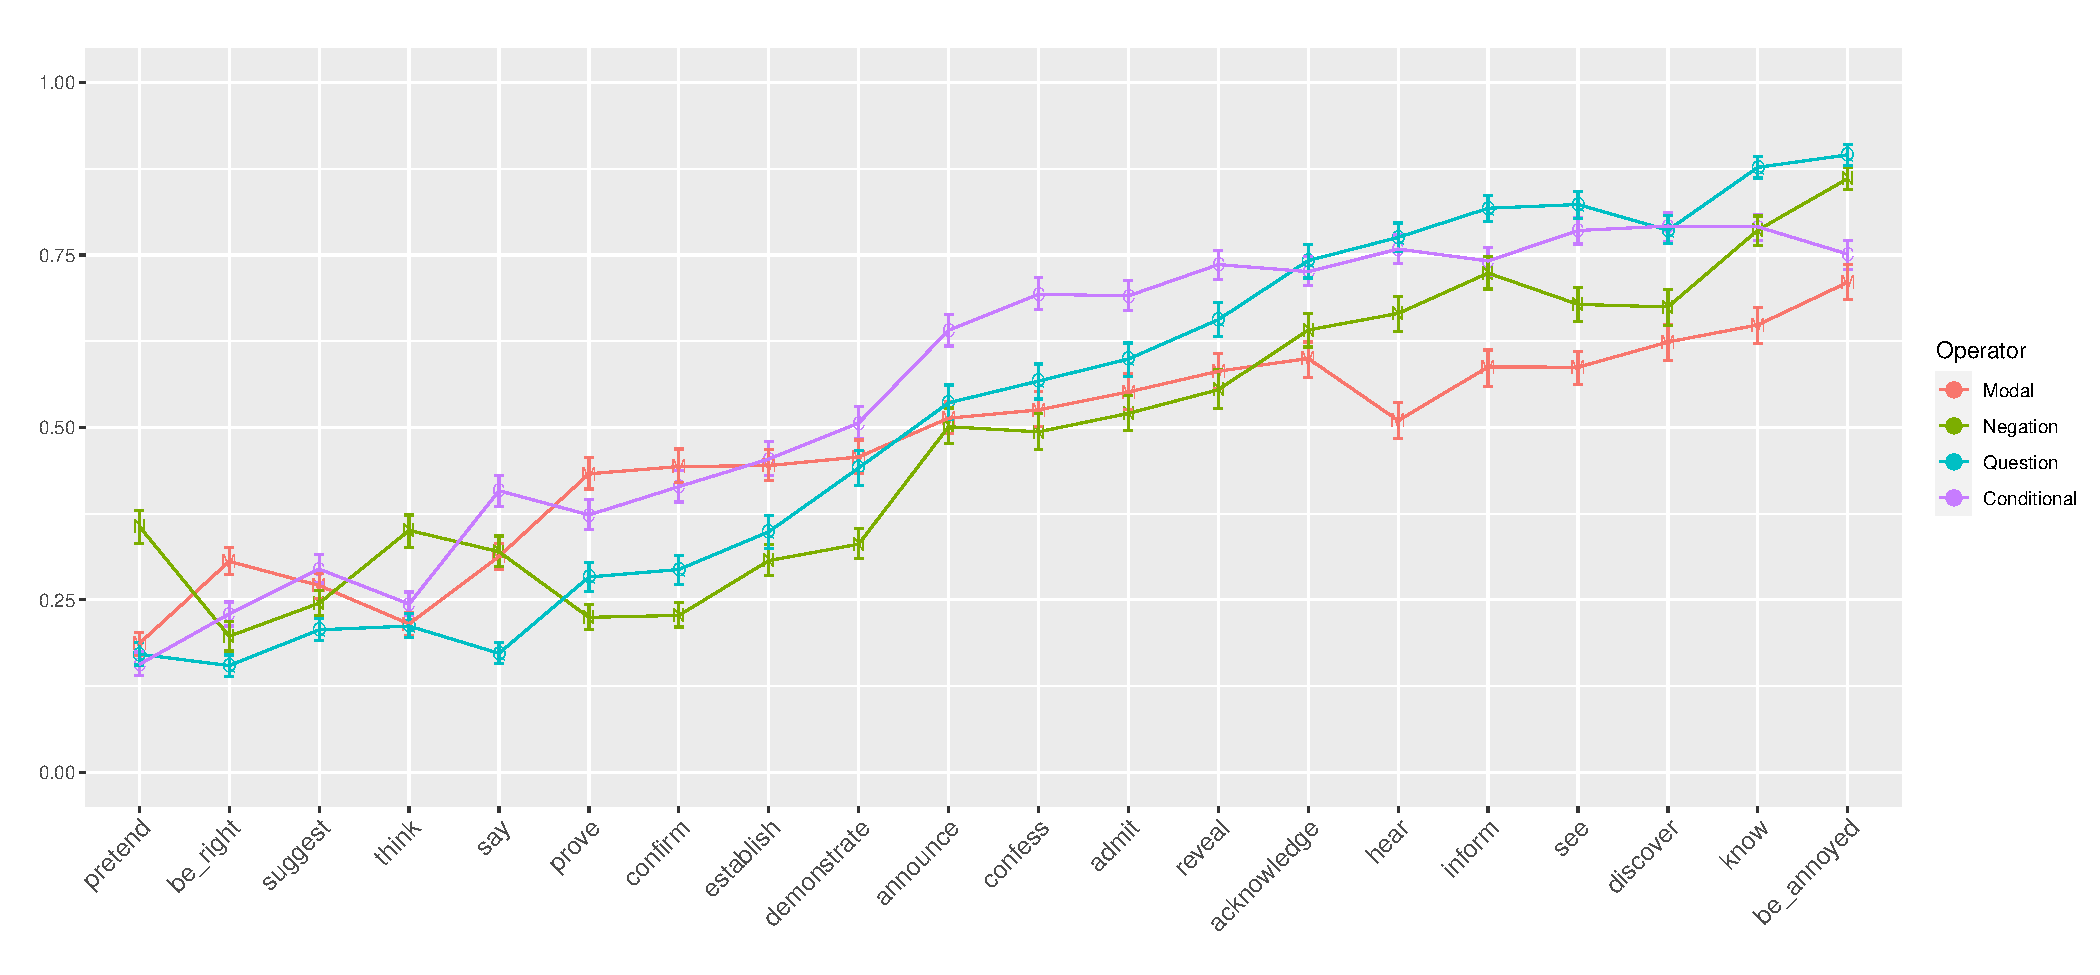
\includegraphics[width=\textwidth]{graphs/proj-by-both.pdf}\vspace{-1.2\baselineskip}
		\caption{\small Mean certainty ratings by predicate and operator}
		\label{fig:figure1}
	\end{figure}

	\vspace{-.3\baselineskip}
	% \textbf{version w baseline know/m}
	% \noindent The data was analyzed using a mixed effects linear regression (using \texttt{lme4, lmertest} in \texttt{R}; \citealp{bates_fitting_2015,kuznetsova_lmertest_2016,r_core_team_r_2014}), with \texttt{know} and \texttt{modal} as reference levels, and random intercepts for participants and items. We found highly significant main effects of \texttt{operator} (\texttt{conditional}: $+0.142$, \texttt{negation}: $+0.143$, ; \texttt{question}: $+0.225$, where $p < 2e^{-16}$ in all three cases), as well as many interactions of \texttt{operator} and  \texttt{verb} across the board (where $p < 0.001$ in $38$ cases, $p < 0.01$ in one, and $p < 0.05$ in three out of $57$ possible interactions).\\

	\noindent The data was analyzed using a mixed effects linear regression (using \texttt{lme4, lmertest} in \texttt{R}; \citealp{bates_fitting_2015,kuznetsova_lmertest_2016,r_core_team_r_2014}), with \texttt{be annoyed} and \texttt{negation} as reference levels, and random intercepts for participants and items. The mean for this baseline (intercept) is $0.867$. We found highly significant main effects of \texttt{operator} for \texttt{conditional} ($-0.116$, $p < 1.6e^{-13}$) and \texttt{modal} ($-0.156$, $p < 2e^{-16}$), while the effect of \texttt{question} was only marginally significant ($+0.025$, $p < 0.1$). We also found many interactions of \texttt{operator} and \texttt{verb} across the board (where $p < 0.001$ in $43$ cases, $p < 0.01$ in three, and $p < 0.05$ in one out of $57$ possible interactions).\\

	Notably, the interactions of:
	\begin{itemize}
		\item discover and question, conditional: significant positive interaction effects (can we really argue that for discover: $Q, C > N$, based on this? I am not really sure how to do this. what I would normally do instead is to look at the posterior samples in a bayesian model to compare each condition and see if they are really different, for $Q, C > N$)

		\item know and question, modal: how can we make argument from model output to differences seen in graph ($Q > C, N > M$)

	\end{itemize}
	
% paragraph method (end)

\paragraph{Discussion and Conclusion.} % (fold)
	\begin{itemize}
		\item Main effect of operator: choice of operator has an effect on projectivity
		\item For \emph{be annoyed}, no significant effect is found for \texttt{question} (vs \texttt{negation}), as would be expected based on Karttunen, but we do find unexpected differences between $N > C, M$ 
		\item for \emph{discover}, we find $Q, C > N$, an effect in the opposite direction from expectation based on Karttunen
		\item \emph{know} shows effects that would be incompatible with characterization as factive or semi-factive: $Q > C, N > M$. if semi-factive, we would expect $N > C, Q$, if factive, no difference would be expected
	\end{itemize}
% paragraph method (end)

\pagebreak
\bibliography{projective-content.bib}

\end{document}